%mm4 comments/revisions on v8 labeled with %mm4
%mm5 revisions on v10 labeled with %mm5
%
\documentclass[useAMS,usenatbib]{mnras}
\topmargin -1cm
\usepackage{graphicx}
\usepackage{textcomp}
\usepackage{amssymb}\usepackage{hyperref}
\usepackage{amsmath,alltt}                                                                                                                     
\usepackage{multirow}
\usepackage{rotating}
\usepackage{lscape}
\usepackage{times}
\usepackage{hyperref}
\usepackage{pdflscape}
\usepackage{supertabular}


%%%%% AUTHORS - PLACE YOUR OWN MACROS HERE %%%%%%%%%%%%%%%%%%%%%%%%%%%%%%%%%%%%%%%%%%%%%%%%%%%%%

\newcommand\lsim{\mathrel{\rlap{\lower4pt\hbox{\hskip1pt$\sim$}}
        \raise1pt\hbox{$<$}}}
\newcommand\gsim{\mathrel{\rlap{\lower4pt\hbox{\hskip1pt$\sim$}}
        \raise1pt\hbox{$>$}}}
\newcommand{\be}{\begin{equation}}
\newcommand{\ba}{\begin{eqnarray}}
%\newcommand{\baa}{\begin{align}}
\newcommand{\ee}{\end{equation}}
\newcommand{\ea}{\end{eqnarray}}
%\newcommand{\eaa}{\end{align}}

%\newcommand{\mnras}{\textrm{MNRAS}}
%\newcommand{\apj}{\textrm{ApJ}}
%\newcommand{\aap}{\textrm{A\&A}}
%\newcommand{\apjl}{\textrm{ApJ}}
%\newcommand{\prd}{\textrm{Phys Rev D}}


\newcommand{\comment}{\bf}
\newcommand{\pont}{{\,^\ast\!}R\,R}
\newcommand{\red}{\color{red}}
\newcommand{\blue}{\color{blue}}
\newcommand{\green}{\color{green}}
\newcommand{\black}{\color{black}}
\newcommand{\Scri}{{\mathcal I}}
\newcommand{\re}{{\textrm{real}}}
\newcommand{\eff}{{\textrm{eff}}}
\newcommand{\p}{{\textrm{pole}}}
\newcommand{\lf}{{\textrm{log-fac}}}
\newcommand{\SMBH}{\bullet}
\newcommand{\SCO}{\star}
\newcommand{\GW}{{\mbox{\tiny GW}}}
\newcommand{\vac}{{\mbox{\tiny vac}}}
\newcommand{\SPA}{{\mbox{\tiny SPA}}}
\newcommand{\Tot}{{\mbox{\tiny tot}}}
\newcommand{\Bondi}{{\mbox{\tiny Bondi}}}
\newcommand{\Ho}{{\mbox{\tiny Hor}}}
\newcommand{\Pa}{{\mbox{\tiny Pade}}}
\newcommand{\pd}{{\mbox{\tiny PD}}}
\newcommand{\Newt}{{\mbox{\tiny Newt}}}
\newcommand{\Pert}{{\mbox{\tiny Pert}}}
\newcommand{\Ta}{{\mbox{\tiny Tay.}}}
\newcommand{\lfac}{{\mbox{\tiny log-fac}}}
\newcommand{\NS}{{\mbox{\tiny NS}}}
\newcommand{\Edd}{{\mbox{\tiny Edd}}}
\newcommand{\Sp}{{\mbox{\tiny S}}}
\newcommand{\ISCO}{{\mbox{\tiny ISCO}}}
\newcommand{\initial}{{\mbox{\tiny Initial}}}
\newcommand{\final}{{\mbox{\tiny Final}}}
\newcommand{\mock}{{\mbox{\tiny mock}}}
\newcommand{\ny}[1]{\textcolor{red}{\it{\textbf{ny: #1}}} }
\newcommand{\sah}[1]{\textcolor{magenta}{\it{\textbf{sah: #1}}} }
\newcommand{\bk}[1]{\textcolor{blue}{\it{\textbf{bk: #1}}} }
\newcommand{\OrbitalFreq}{\Omega}
\newcommand{\Sm}{{\mbox{\tiny S}}}
\newcommand{\La}{{\mbox{\tiny L}}}
\newcommand{\EOB}{{\mbox{\tiny EOB}}}
\newcommand{\Msun}{\,{\rm M_\odot}}
\newcommand{\yr}{\,{\rm yr}}
\newcommand{\cm}{\,{\rm cm}}
\newcommand{\gm}{\,{\rm g}}
\newcommand{\I}{\mathcal{J}}
\newcommand{\D}{\mathrm{d}}
\newcommand{\orb}{\mathrm{orb}}
\newcommand{\R}{{\bar{r}}}
\newcommand{\Ls}{\ell}
\newcommand{\gas}{\mathrm{gas}}
\newcommand{\gap}{\mathrm{gap}}
\newcommand{\dL}{d_{\rm L}}

%\newcommand{\mnras}{\textrm{MNRAS}}
%\newcommand{\apj}{\textrm{ApJ}}
%\newcommand{\aap}{\textrm{A\&A}}
%\newcommand{\apjl}{\textrm{ApJ}}


\title[Compact Binaries of BS Twins from Stellar Triples]{A Triple Origin for Twin Blue Stragglers in Compact Binaries}

\author[N. W. C. Leigh \& S. Portegies Zwart]{N. W. C. Leigh$^{1,2,3}$, S. Portegies Zwart$^{4}$ \\
$^{1}$Department of Astrophysics, American Museum of Natural History, New York, NY 10024, USA\\
$^{2}$Department of Physics and Astronomy, Stony Brook University, Stony Brook, NY 11794-3800, USA\\
$^{3}$Center for Computational Astrophysics, Flatiron Institute, 162 Fifth Avenue, New York, NY 10010, USA\\
$^{4}$Leiden Observatory, }

\begin{document}

\date{Accepted. Received; in original form}

\pagerange{\pageref{firstpage}--\pageref{lastpage}} \pubyear{2008}

\maketitle

\label{firstpage}

\begin{abstract}
In this Letter, we propose a potential formation mechanism for twin blue stragglers in compact binaries that involves mass transfer from an evolved outer tertiary companion on to the inner binary via a circumbinary disk.  We apply our hypothetical scenario to the observed double blue straggler system Binary 7782 in the old open cluster NGC 188, and show that its observed properties are easily and even naturally reproduced within the context our proposed model.  Within the context of the hypothetical formation mechanism proposed here, the presented work predicts the following properties for the post-mass transfer double BS tertiary:  (1)  For the outer tertiary orbit, the semi-major axis should lie between 2 AU $\lesssim$ a$_{\rm out}$ $\lesssim$ 5 AU, assuming initial masses for the inner binary components of m$_{\rm 1} =$ 1.1 M$_{\odot}$ and m$_{\rm 2} =$ 0.9 M$_{\odot}$ and an outer tertiary mass of m$_{\rm 3} =$ 1.4 M$_{\odot}$. (2)  Larger final WD masses, and hence core masses for the donor at the time of mass transfer, should correspond to larger final outer orbital periods for the tertiary. (3)  For the inner binary, the rotational axes of the BSs should be aligned with each other and the orbital plane of the outer tertiary WD. (4)  The BSs in the inner binary should have roughly equal masses, independent of their initial masses.  This predicts that the initially lower mass MS star should accrete the most, and should hence be polluted more significantly by any accreted material.  This could be observable in the surface layers of a radiative star (i.e., He, C and O if the donor is an RGB star, and/or s-process elements if the donor is an AGB star). (5) Twin BSs in compact binaries formed from the proposed mechanism should be more frequent in younger clusters with ages $\lesssim$ 4-6 Gyr, since the donor will have  radiative envelope.

\end{abstract}

\begin{keywords}
stars: blue stragglers -- binaries: general -- globular clusters: general -- scattering. 
\end{keywords}

%%%%%%%%%%%%%%%%%%%%%%%%%%%%%%%
\section{Introduction}

Blue straggler (BS) stars appear brighter and bluer than the main-sequence turn-off (MSTO) in a cluster colour-magnitude diagram (CMD).  Two primary channels for BS formation have been proposed; mass transfer from an evolved donor on to a main-sequence star in a binary star system \citep[e.g.][]{mccrea64,knigge09,leigh11,gosnell14,gosnell15}, and direct stellar collisions involving main-sequence stars mediated via direct interactions involving binaries \citep[e.g.][]{hills75,shara97,leigh13,hypki13}.  Other possible, albeit related, formation mechanisms include mergers of compact MS-MS binaries, and mergers of the inner MS-MS binaries of hierarchical triple star systems induced by Lidov-Kozai oscillations coupled with tidal damping \citep[e.g.][]{perets09}.  

In spite of these specific predictions for the expected properties of BSs formed from each of the above production mechanisms, there exist many BSs with observed properties that defy these simple scenarios.  For example, in the old open cluster M67, there lurks a candidate triple system that is posited to host \textit{two} BSs \citep{vandenberg01,sandquist03}.  The observations suggest that the outer tertiary is itself a BS, with a mass $\sim$ 1.7 M$_{\odot}$ and orbiting the inner binary with a period of 1188.5 days \citep{sandquist03}.  The inner binary has a period of only 1.068 days \citep{vandenberg01}, and hosts a BS of mass 2.52 M$_{\odot}$.  Thus, in order to form this system after convolving its observed properties with its host cluster age, we require at least five stars in order to conserve the total system mass \citep{leigh11}.  As explained in \citet{leigh11}, this is strongly indicative of a dynamical origin for the system, and a single direct interaction involving a binary and a triple that resulted in two separate collision events is the most probable explanation for its origin (i.e., a single interaction involving two multiples with two or more stars is a more likely scenario to produce this system than two back-to-back direct binary-binary interactions).  

Even more curious, there exists in the old open cluster NGC 188 a double BS binary, called Binary 7782.  Specifically, \citet{mathieu09} observed a compact and mildly eccentric (i.e., e $\sim$ 0.1) binary star system with an orbital period of $\sim$ 10 days hosting \textit{two} blue stragglers.  During a given binary-binary interaction, the probability that not one but \textit{two} direct MS-MS collisions occur is less than a percent \citep{leonard89,leigh11,leigh12}.  Typically, such binaries are very wide with long orbital periods.  Thus, dynamically, it is very difficult to form a compact binary composed of two collision products during a single direct interaction in a star cluster.  So, how did Binary 7782 form?  MENTION BIMODAL P-E DISTRIBUTION, AND HOW THIS COULD BE SUGGESTIVE OF A TRIPLE ORIGIN FOR SOME OF THE SUBSET OF OBSERVED BSs.

In this Letter, we propose a potential formation channel for Binary 7782, and compact double BS binaries in general, which involves mass transfer from an outer tertiary companion on to an inner MS-MS binary.  In section~\ref{dyn}, we constrain the range of present-day orbital parameters for a hypothetical outer tertiary companion, using a combination of dynamical and stellar evolution-based constraints.  In Section~\ref{sims} we present the numerical simulations used to study the mass transfer process in our hypothetical triple system, computed using the \texttt{AMUSE} software package, in order to study the evolution of the inner and outer orbital parameters during mass transfer.  We summarize and discuss the implications of our results for compact double BS binaries and, more generally, mass transfer in stellar triples in Section~\ref{discussion}.  

\section{Constraints on the present-day orbital parameters for a hypothesized tertiary companion in the compact BS Binary 7782} \label{dyn}

Consider a hierarchical triple system with component masses m$_{\rm 1}$ and m$_{\rm 2}$ for the inner binary, and mass m$_{\rm 3}$ for the outer tertiary companion.  The inner and outer binary orbital semi-major axes are denoted a$_{\rm in}$ and a$_{\rm out}$, respectively.  We assume circular orbits for both the inner and outer orbits.  

We consider a scenario where the outer tertiary companion is filling its Roche lobe and is hence transferring mass to the inner binary.  Using conservation of angular momentum, we can equate the specific angular momentum of the accreted mass at the inner Lagrangian point of the donor star to the final specific angular momentum of the accretion stream at the circularization radius about the inner binary:
\begin{equation}
\label{eqn:specangmom1}
v_{\rm orb,3}(a_{\rm out} - r_{\rm L}) = v_{\rm orb,c}a_{\rm c},
\end{equation}
where R$_{\rm L}$ is the radius of the Roche lobe of the outer tertiary companion, a$_{\rm c}$ is the semi-major axis of the orbit about the inner binary corresponding to the circularization radius and v$_{\rm orb,c}$ is the orbital velocity at a$_{\rm c}$.  The distance from the center of mass corresponding to the outer tertiary companion defined by the Roche lobe is given by \citep{eggleton83}: 
\begin{equation}
\label{eqn:roche}
R_{\rm L} = \frac{0.49q^{2/3}}{0.6q^{2/3} + {\rm ln}(1 + q^{1/3})}a_{\rm out},
\end{equation}
where the mass ratio q is defined as q $=$ m$_{\rm 3}$/(m$_{\rm 1} +$ m$_{\rm 2}$).  Combining Equation~\ref{eqn:roche} with Equation~\ref{eqn:specangmom1}, we can solve for the circularization radius as a function of a$_{\rm out}$ and the assumed stellar masses:
\begin{equation}
\label{eqn:ac}
a_{\rm c} = a_{\rm out}(1 - R_{\rm L}).
\end{equation}
In order for a circumbinary disk to form around the inner binary, we require that a$_{\rm in} <$ a$_{\rm c}$.

Figure~\ref{fig:fig1} shows the parameter space in the a$_{\rm out}$-a$_{\rm in}$-plane for Binary 7782.  We assume initial component masses of m$_{\rm 1}$ = 1.1 M$_{\rm \odot}$ and m$_{\rm 2}$ = 0.9 M$_{\rm \odot}$ for the inner binary components, and m$_{\rm 3}$ = 1.4 M$_{\rm \odot}$ for the outer tertiary.  This choice is guided by the current turn-off mass of 1.1 M$_{\odot}$ in NGC 188 \citep{mathieu09} and a maximum BS age of a few Gyr \citep[e.g.][]{sills99,sills01}.  After comparing the circularization radius to the semi-major axis of the inner binary and folding in all constraints from the requirements for dynamical stability, an outer tertiary that is Roche lobe-filling, and a dynamically hard outer tertiary orbit.  The thick horizontal solid red line shows the allowed range of outer semi-major axes allowed, after folding in all of the aforementioned criteria.  As is clear, this makes a relatively narrow prediction for the allowed ranges of outer tertiary orbits, namely 2 AU $\le$ a$_{\rm out} \le$ 5 AU.  

\begin{figure}
\begin{center}
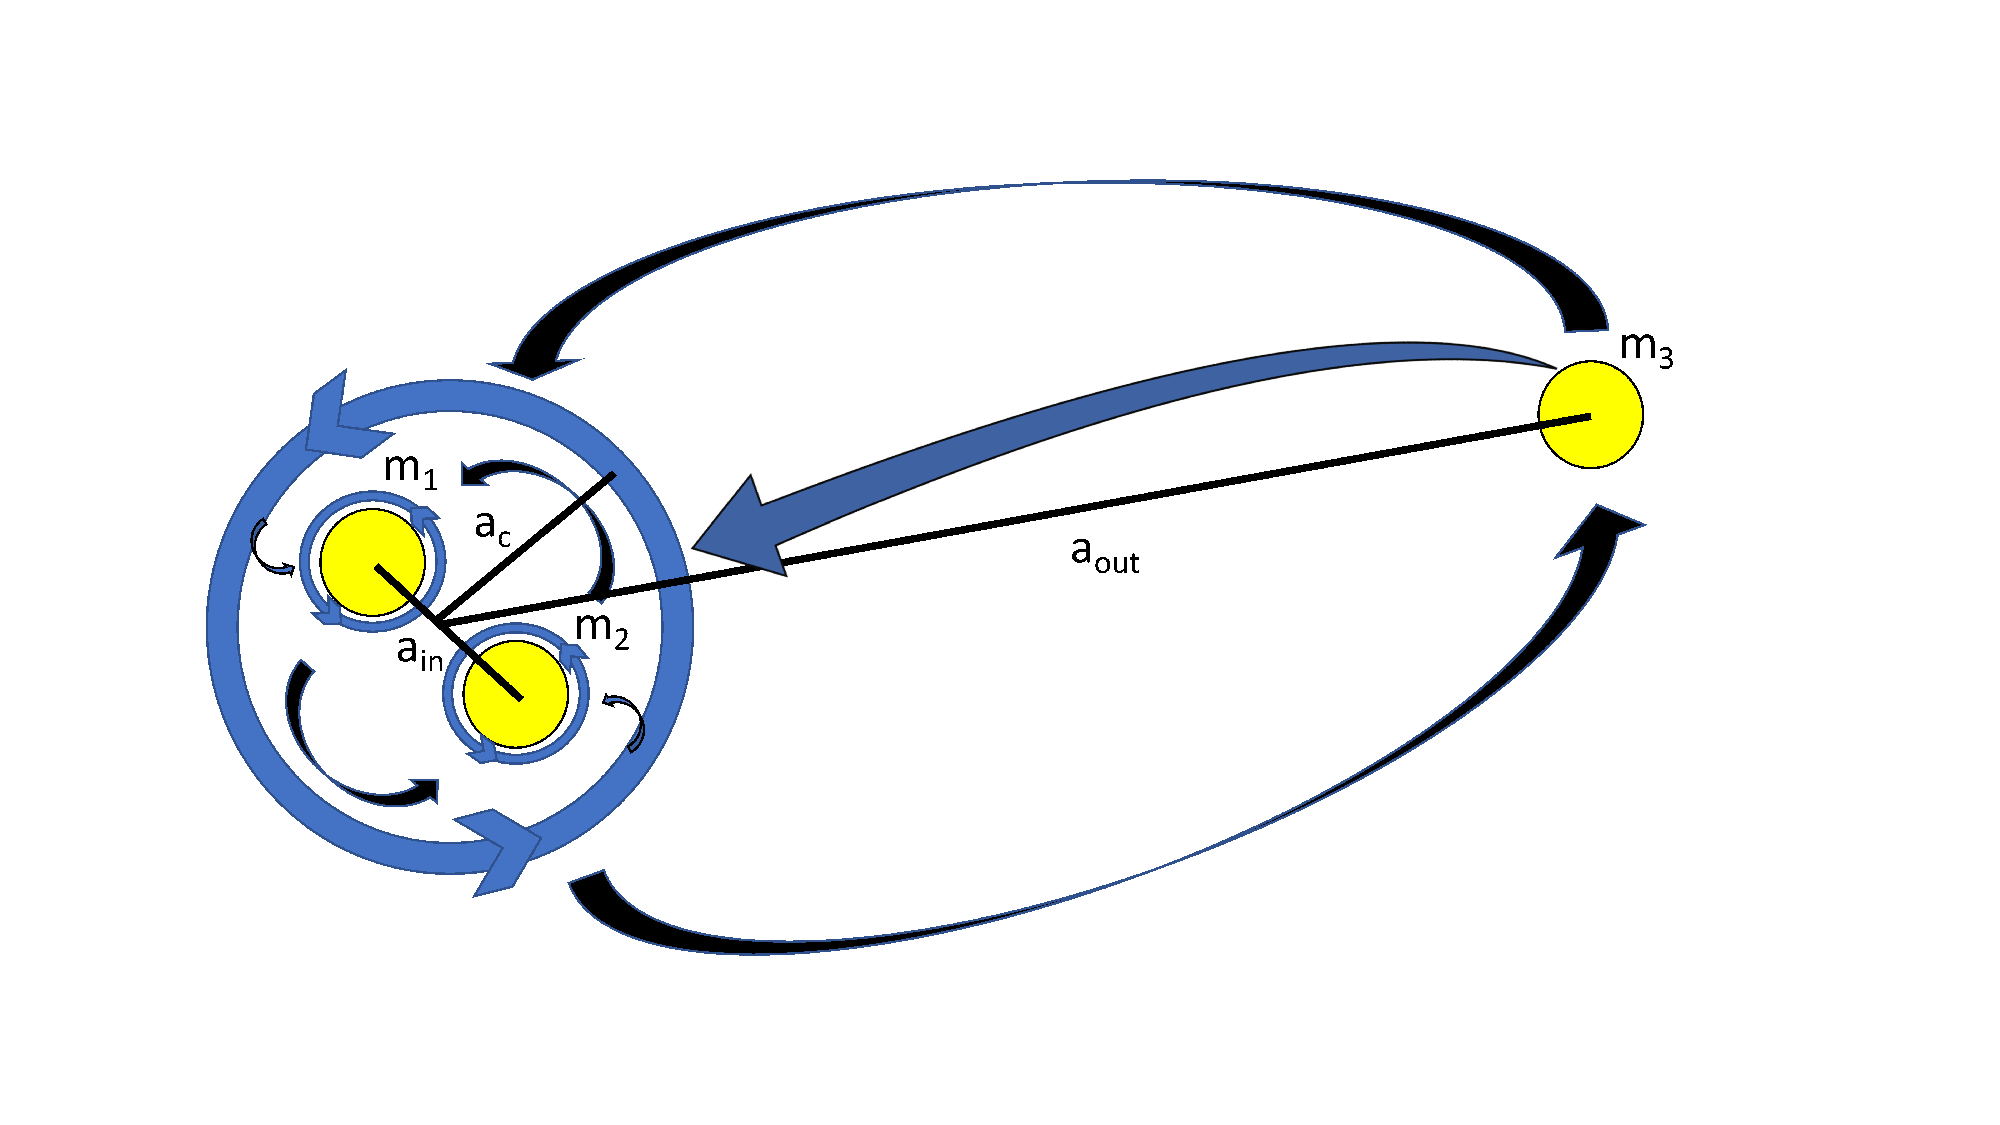
\includegraphics[width=\columnwidth]{fig1.eps}
\end{center}
\caption[Parameter space in the a$_{\rm out}$-a$_{\rm in}$-plane allowed for the hypothetical outer tertiary orbit of Binary 7782.]{Parameter space in the a$_{\rm out}$-a$_{\rm in}$-plane allowed for the hypothetical outer tertiary orbit of Binary 7782.  The solid diagonal black lines show the circularization radius a$_{\rm c}$ for the mass transfer stream coming from the outer tertiary, for different values of the mas ratio, namely q $=$ 0.1, 0.5, 1, 2 and 10.  We assume initial component masses of m$_{\rm 1}$ = 1.1 M$_{\rm \odot}$ and m$_{\rm 2}$ = 0.9 M$_{\rm \odot}$ for the inner binary components, and m$_{\rm 3}$ = 1.4 M$_{\rm \odot}$ for the outer tertiary.  We assume completely conservative mass transfer for this exercise, and a final mass for the outer tertiary of 0.6 M$_{\rm \odot}$ once it has become a WD.  The dashed diagonal black line shows a rough criterion for dynamical stability in the triple, roughly following \citet{mardling99} (i.e., a$_{\rm in} <$ 0.1a$_{\rm out}$ is required).  The vertical solid red lines show the outer semi-major axes corresponding to the hard-soft boundary assuming central velocity dispersions of $\sigma =$ 1, 5 and 10 km s$^{-1}$.  The vertical dashed black lines show the maximum outer semi-major axis a$_{\rm out}$ for which the outer tertiary companion is Roche lobe-filling, assuming a stellar radius of R$_{\rm 3} =$ 200 R$_{\odot}$ (CHANGE).  The horizontal solid red line shows the semi-major axis corresponding to a contact state for the inner binary, assuming R$_{\rm 1} =$ R$_{\rm 2} =$ 1 R$_{\odot}$.  The horizontal dashed red line shows the observed semi-major axis for Binary 7782, for our assumed final inner companion masses (i.e., m$_{\rm 1} =$ m$_{\rm 2} =$ 1.4 M$_{\odot}$).  Finally, the thick solid horizontal red line shows the parameter space for a$_{\rm out}$ allowed after considering all of the aforementioned criteria.
\label{fig:fig1}}
\end{figure}

\section{Numerical Simulations} \label{sims}

\subsection{AMUSE} \label{amuse}

We use smoothed-particle hydrodynamics (SPH) simulations to compute the time evolution of the mass transfer process.  

\subsection{Initial Conditions} \label{ICs}

In this section, we describe and justify our choice of initial conditions for both our analytic calculations and smoothed-particle hydrodynamics simulations.

We adopt initial component masses of m$_{\rm 1}$ = 1.1 M$_{\rm \odot}$ and m$_{\rm 2}$ = 0.9 M$_{\rm \odot}$ for the inner binary components, and m$_{\rm 3}$ = 1.4 M$_{\rm \odot}$ for the outer tertiary.  This choice for the initial mass of the outer tertiary is critical since it ensures that the donor star during the mass transfer process will have a radiative envelope \citep[e.g.][]{maeder09}.  In turn, this ensures that the mass transfer will be maximally conservative, such that the accretion stream will be maximally stable, accreting at a stable and constant rate \citep[e.g.][]{iben91}.  

\section{Results} \label{results}


\section{Summary and Discussion} \label{discussion}

In this Letter, we have proposed a formation scenario for double BS equal-mass compact binaries, as observed for Binary 7782 in the old open cluster NGC 188.  The proposed scenario involves mass transfer from an evolved outer tertiary companion, which is accreted by the inner binary via a circumbinary disk.  Our scenario makes several predictions for the observed properties of a hypothetical outer triple companion, now a WD.  These are:

\begin{enumerate}

\item For the outer tertiary orbit, the semi-major axis should lie between 2 AU $\lesssim$ a$_{\rm out}$ $\lesssim$ 5 AU, assuming initial masses for the inner binary components of m$_{\rm 1} =$ 1.1 M$_{\odot}$ and m$_{\rm 2} =$ 0.9 M$_{\odot}$ and an outer tertiary mass of m$_{\rm 3} =$ 1.4 M$_{\odot}$.

\item Larger final WD masses, and hence core masses for the donor at the time of mass transfer, should correspond to larger final outer orbital periods for the tertiary.  This is because the Roche radius is larger for larger outer orbital periods, such that the donor must evolve to larger radii, and hence core masses, before the onset of mass transfer.

\item For the inner binary, the rotational axes of the BSs should be aligned with each other and the orbital plane of the outer tertiary WD.  This is because accretion onto the BS progenitors proceeds via an accretion disk, that forms at the circularization radius and that has an orbital plane aligned with that of the outer tertiary.

\item The BSs in the inner binary should have roughly equal masses, independent of their initial masses.  This is because it is the lowest mass object that typically accretes the fastest, since its orbital velocity and distance relative to the circumbinary disk is typically the lowest.  This quickly brings the mass ratio toward unity.  This predicts that the initially lower mass MS star should accrete the most, and should hence be polluted more significantly by any accreted material.  This could be observable in the surface layers of a radiative star.  If the donor is an RGB star, the accretor will be enriched in mostly carbon, oxygen and helium.  If the accretor is an AGB star, it will be enriched in mostly s-process elements.

\item Twin BSs in compact binaries formed from the proposed mechanism should be more frequent in younger clusters with ages $\lesssim$ 4-6 Gyr.  This is because clusters with a main-sequence turn-off mass $\lesssim$ 1.2 M$_{\odot}$ have convective envelopes \citep[e.g.][]{iben91,maedoer09}, and a radiative envelope for the donor in a mass transferring binary ensures stable accretion on to the accretor.

WHAT ELSE?  SOMETHING RELATED TO TIMESCALES AND THE PROBABiLitY OF OBSERVING THE WD?

\end{enumerate}


\section{Acknowledgments}

N.W.C.L. acknowledges support from a Kalbfleisch Fellowship at the American Museum of Natural History.  T.H.P. acknowledges the support through the FONDECYT Regular Project No. 1161817 and the BASAL Center for Astrophysics and Associated Technologies (PFB-06).

\begin{thebibliography}{99}

\bibitem[\protect\citeauthoryear{Anderson et al.}{2008}]{anderson08}
  Anderson J.,  Sarajedini A., Bedin L. R., King I. R., Piotto G.,
  Reid I. N., Siegel M., Majewski S. R., Paust N. E. Q., Aparicio A.,
  Milone A. P., Chaboyer B., Rosenberg A. 2008, AJ, 135, 2055
\bibitem[\protect\citeauthoryear{Artymowicz et al.}{1993}]{artymowicz93} Artymowicz P., Lin D. N. C., Wampler E. J. 1993, ApJ, 409, 592 
%\bibitem[\protect\citeauthoryear{Bartos et al.}{2017}]{Bartos17} Bartos I., Kocsis B., Haiman Z. \& M\'{a}rka S., 2017, ApJ, 835, 165
%\bibitem[\protect\citeauthoryear{Bartko et al.}{2009}]{Bartko09} Bartko H., Martins F., Trippe S., Fritz T. K., Genzel R., Ott T., Eisenhauer F., Gillessen S., Paumard T., Alexander T., Dodds-Eden K., Gerhard O., Levin Y., Mascetti L., Nayakshin S., Perets H. B., Perrin G., Pfuhl O., Reid M. J., Rouan D., Sternberg A., Trippe S., 2009, ApJ, 697, 1741
%\bibitem[\protect\citeauthoryear{Bartko et al.}{2010}]{Bartko10} Bartko H., Martins F., Fritz T. K., Genzel R., Levin Y., Perets H. B., Paumard T., Nayakshin S., Gerhard O., Alexander T., Dodds-Eden K., Eisenhauer F., Gillessen S., Mascetti L., Ott T., Perrin G., Pfuhl O., Reid M. J., Rouan D., Zilka M., Sternberg A., 2010, ApJ, 708, 834
%\bibitem[\protect\citeauthoryear{Baruteau et al.}{2011}]{Baruteau11} Baruteau C., Cuadra J. \& Lin D.N.C., 2011, ApJ, 726, 28
\bibitem[\protect\citeauthoryear{Bedin et al.}{2010}]{bedin10} Bedin L. R., Cassisi S., Castelli F., Piotto G., Anderson J., Salaris M., Momany Y., Pietrinferni A. 2010, MNRAS 357, 1038
%\bibitem[\protect\citeauthoryear{Bender et al.}{2005}]{bender05} Bender R., Kormendy J., Bower G., et al. 2005, ApJ, 631, 280
\bibitem[\protect\citeauthoryear{Bruzual \& Charlot}{2003}]{bruzual03} Bruzual G., Charlot S. 2003, MNRAS, 344, 1000 
\bibitem[\protect\citeauthoryear{Casassus et al.}{2013}]{casassus13} Casassus S., Hales A., de Gregorio I., Dent B., Belloche A., G\:usten R., M\'enard F., Hughes A. M., Wilner D., Salinas V. 2013, A\&A, 553, 64 
\bibitem[\protect\citeauthoryear{Ceillier et al.}{2017}]{ceillier17} Ceillier T., Tayar J., Mathur S., Salabert D., Garc\'ia R. A., Stello D., Pinsonneault M. H., van Sanders J., Beck P. G., Bloemen S. 2017, A\& A, 605, 111 
\bibitem[\protect\citeauthoryear{Chatterjee et al.}{2013}]{chatterjee13} Chatterjee S., Rasio F. A., Sills A., Glebbeek E. 2013, ApJ, 777, 106  
%\bibitem[\protect\citeauthoryear{Chen \& Amaro-Seoane}{2015}]{chen15} Chen X., Amaro-Seoane P. 2015, Classical and Quantum Gravity, 32, 6 
\bibitem[\protect\citeauthoryear{Dotter et al.}{2010}]{dotter10} Dotter, A., Sarajedini A., Anderson J., Aparicio A., Bedin L. R., Chaboyer B., Majewski S., Marin-Franch A., Milone A., Paust N., Piotto G., Reid N., Rosenberg A., Siegel M. 2010, ApJ 708, 698

\bibitem[\protect\citeauthoryear{Dalessandro et al.}{2013}]{dalessandro13} Dalessandro E., Ferraro F. R., Massari D., Lanzoni B., Miocchi R. P., Beccari G., Bellini A., Sills A., Sigurdsson S., Mucciarelli A., Lovisi L. 2013, ApJ, 778, 135
\bibitem[\protect\citeauthoryear{Eggleton}{1983}]{eggleton83} Eggleton P. P. 1983, ApJ, 268, 368 
\bibitem[\protect\citeauthoryear{Flock et al.}{2015}]{flock15} Flock M., Ruge J. P., Dzyurkevich N., Henning Th., Klahr H., Wolf S. 2015, A\&A, 574, 68
\bibitem[\protect\citeauthoryear{Ferraro et al.}{1997}]{ferraro97}
  Ferraro F. R., Paltrinieri B., Fusi Pecci F., Cacciari C., Dorman
  B., Rood R. T., Buonanno R., Corsi C. E., Burgarella D., Laget
  M. 1997, A\&A, 324, 915
\bibitem[\protect\citeauthoryear{Ferraro et al.}{1999}]{ferraro99}
  Ferraro F. R., Paltrinieri B., Rood R. T., Dorman B. 1999, ApJ, 522,
  983
\bibitem[\protect\citeauthoryear{Ferraro et al.}{2004}]{ferraro04}
  Ferraro F. R., Beccari G., Rood, R. T., Bellazzini M., Sills A.,
  Sabbi E. 2004, ApJ, 603, 127
\bibitem[\protect\citeauthoryear{Ferraro, Valenti \& Origlia}{2006}]{ferraro06} Ferraro F. R., Valenti E., Origlia L. 2006, ApJ, 649, 243
\bibitem[\protect\citeauthoryear{Ferraro et al.}{2009}]{ferraro09} Ferraro F. R., Beccari G., Dalessandro E., Lanzoni B., Sills A., Rood R. T., Pecci F. F., Karakas A. I., Miocchi P., Bovinelli S. 2009, Nature, 462, 1028  
\bibitem[\protect\citeauthoryear{Fregeau et al.}{2004}]{fregeau04} Fregeau J. M., Cheung P.,
  Portegies Zwart S. F., Rasio F. A. 2004, MNRAS, 352, 1
\bibitem[\protect\citeauthoryear{Fregeau, Ivanova \& Rasio}{2009}]{fregeau09} Fregeau J. M., Ivanova N.,
  Rasio F. A. 2009, ApJ, 707, 1533
%\bibitem[\protect\citeauthoryear{Geller at al.}{2009}]{geller09}
%  Geller A. M., Mathieu R. D., Harris H. C., McClure R. D., 2009,
%  AJ, 137, 3743
\bibitem[\protect\citeauthoryear{Geller \& Mathieu}{2011}]{geller11}
  Geller A. M., Mathieu R. D. 2011, Nature, 478, 356
\bibitem[\protect\citeauthoryear{Geller \& Mathieu}{2012}]{geller12} Geller A. M., Mathieu R. D. 2012, AJ, 144, 54
\bibitem[\protect\citeauthoryear{Geller et al.}{2013a}]{geller13a} Geller A. M.,
de Grijs R., Li C., Hurley J. R. 2013, ApJ, 779, 30
\bibitem[\protect\citeauthoryear{Geller et al.}{2013b}]{geller13b} Geller A. M., Hurley J. R., Mathieu R. D. 2013, AJ, 145, 8
\bibitem[\protect\citeauthoryear{Geller \& Leigh}{2015}]{geller15} Geller A. M., Leigh W. W. C. 2015, ApJL, 808, L25 
%\bibitem[\protect\citeauthoryear{Ghez}{2008}]{ghez08} Ghez A. M., Salim S., Weinberg N. N., Lu J. R., Do T., Dunn J. K., Matthews K, Morris M. R., Yelda S., Becklin E. E., Kremenek T., Milosavlevic M., Naiman J., ApJ, 2008, 689, 1044 
%\bibitem[\protect\citeauthoryear{Ghez}{2008}]{ghez08}
\bibitem[\protect\citeauthoryear{Gosnell et al.}{2014}]{gosnell14} Gosnell N. M., Mathieu R. D., Geller A. M., Sills A., Leigh N. W. C., Knigge C. 2014, ApJ, 783, 8
\bibitem[\protect\citeauthoryear{Gosnell et al.}{2015}]{gosnell15} Gosnell N. M., Mathieu R. D., Geller A. M., Sills A., Leigh N. W. C., Knigge C. 2015, ApJ, 814, 163
%\bibitem[\protect\citeauthoryear{Graham \& Spitler}{2009}]{Graham09} Graham A.W. \& Spitler L.R., 2009, MNRAS, 397, 2148
\bibitem[\protect\citeauthoryear{Harris et al.}{1996; 2010 update}]{harris96} Harris W. E. 1996, AJ, 112,
  1487; 2010 update
%\bibitem[\protect\citeauthoryear{Heggie}{1975}]{heggie75} Heggie D. C. 1975, MNRAS, 173, 729
\bibitem[\protect\citeauthoryear{Heggie \& Hut}{2003}]{heggie03}
  Heggie D. C., Hut P. 2003, The Gravitational Million-Body Problem:
  A Multidisciplinary Approach to Sar Cluster Dynamics (Cambridge:
  Cambridge University Press)
\bibitem[\protect\citeauthoryear{Hills}{1975}]{hills75} Hills J. G. 1975, AJ, 80, 809
\bibitem[\protect\citeauthoryear{Hurley et al.}{2005}]{hurley05}
  Hurley J. R., Pols O. R., Aarseth S. J., Tout C. A. 2005, MNRAS,
  363, 293
%\bibitem[\protect\citeauthoryear{Hurley, Aarseth \&
%    Shara}{2007}]{hurley07} Hurley J. R., Aarseth S. J., Shara M. M. 2007, ApJ, 665, 707
%\bibitem[\protect\citeauthoryear{Hut \& Bahcall}{1983}]{hut83} Hut P., Bahcall J. N. 1983, ApJ,
%  268, 319
\bibitem[\protect\citeauthoryear{Howarth}{1983}]{howarth83} Howarth I. D. 1983, MNRAS, 203, 301
\bibitem[\protect\citeauthoryear{Hypki \& Giersz}{2013}]{hypki13} Hypki A., Giersz M. 2013,
MNRAS, 429, 1221
\bibitem[\protect\citeauthoryear{Iben}{1991}]{iben91}  Iben I., Jr. 1991, ApJS, 76, 55
\bibitem[\protect\citeauthoryear{Knigge, Leigh \& Sills}{2009}]{knigge09} Knigge C., Leigh
  N., Sills A. 2009, Nature, 457, 288
\bibitem[\protect\citeauthoryear{Laidler et al.}{2008}]{laidler08} Laidler et al. 2008, ``Synphot Data User's Guide'' (Baltimore, STScI)
\bibitem[\protect\citeauthoryear{Lanzoni et al.}{2007}]{lanzoni07} Lanzoni B., Dalessandro E., Ferraro F. R., Valenti E., Beccari G., Schiavon R. P., Rood R. T., Mapelli M., Sigurdsson S. 2007, ApJ, 663, 1040
%\bibitem[\protect\citeauthoryear{Kaluzny et al.}{1998}]{kaluzny98} Kaluzny J., Hilditch R. W., Clement C., Rucinski S. M. 1998, MNRAS, 296, 347
%\bibitem[\protect\citeauthoryear{Kaluzny et al.}{2015}]{kaluzny15} Kaluzny J., Thompson I. B., Narloch W., Pych W., Rozyczka M. 2015, Acta Astronomica, 65, 267 
\bibitem[\protect\citeauthoryear{Leigh, Sills \& Knigge}{2007}]{leigh07} Leigh
  N. W., Sills A., Knigge C. 2007, ApJ, 661, 210
%\bibitem[\protect\citeauthoryear{Leigh, Sills \& Knigge}{2008}]{leigh08} Leigh
%  N. W., Sills A., Knigge C. 2008, ApJ, 678, 564
%\bibitem[\protect\citeauthoryear{Leigh, Sills \& Knigge}{2009}]{leigh09} Leigh
%  N. W., Sills A., Knigge C. 2009, MNRAS, 399, L179
\bibitem[\protect\citeauthoryear{Leigh \& Sills}{2011}]{leigh11} Leigh N., Sills A. 2011, MNRAS, 410, 2370
\bibitem[\protect\citeauthoryear{Leigh et al.}{2012}]{leigh12} Leigh N. W., Umbreit S.,
Sills A., Knigge C., De Marchi G., Glebbeek E., Sarajedini A. 2012, MNRAS, 422, 1592
\bibitem[\protect\citeauthoryear{Leigh et al.}{2013}]{leigh13} Leigh N. W., Knigge C.,
Sills A., Perets H. B., Sarajedini A., Glebbeek E. 2013, MNRAS, 428, 897
%\bibitem[\protect\citeauthoryear{Leigh et al.}{2014}]{leigh14} Leigh N. W. C., L\"utzgendorf N., 
%Geller A. M., Maccarone T. J., Heinke C., Sesana A. 2014, MNRAS, 444, 29
%\bibitem[\protect\citeauthoryear{Leigh et al.}{2016a}]{leigh16a} Leigh N. W. C., Antonini F., Stone N. C., Shara M. M., Merritt D. 2016a, MNRAS, 463, 1605
%\bibitem[\protect\citeauthoryear{Leigh et al.}{2016b}]{leigh16b} Leigh N. W. C., Stone N. C., Geller A. M., Shara M. M., Muddu H., Solano-Oropeza D., Thomas Y. 2016b, MNRAS, 463, 3311 
%\bibitem[\protect\citeauthoryear{Leigh et al.}{2016c}]{leigh16c} Leigh N. W. C., Geller A. M., Toonen S. 2016c, ApJ, 818, 21
%\bibitem[\protect\citeauthoryear{Leigh et al.}{2016d}]{leigh16d} Leigh N. W. C., Shara M. M., Geller A. M. 2016d, MNRAS, 459, 1242
\bibitem[\protect\citeauthoryear{Leonard}{1989}]{leonard89} Leonard
  P. J. T. 1989, AJ, 98, 217
%\bibitem[\protect\citeauthoryear{Leonard \& Linnell}{1992}]{leonard92}
%  Leonard P. J. T., Linnell A. P. 1992, AJ, 103, 1928
%\bibitem[\protect\citeauthoryear{Leonard \& Livio}{1995}]{leonard95} Leonard P. J. T., Livio M. 1995,
%  ApJ, 447, L121
\bibitem[\protect\citeauthoryear{Lim, Diaz \& Laidler}{2015}]{lim15} Lim P. L., Diaz R. L., Laidler V. 2015, PySynphot User's Guide (Baltimore, MD: STScI)
\bibitem[\protect\citeauthoryear{Lovisi et al.}{2012}]{lovisi12} Lovisi L., Mucciarelli A., Lanzoni B., Ferraro F. R., Gratton R., Dalessandro E., Contreras R. R. 2012, ApJ, 754, 91
\bibitem[\protect\citeauthoryear{Maeder}{2009}]{maeder09} Maeder A. 2009, 
Physics, Formation and Evolution of Rotating Stars. Berlin: Springer-Verlag
\bibitem[\protect\citeauthoryear{Mardling \& Aarseth}{1999}]{mardling99} Mardling R. A., Aarseth S. J. 1999, ASIC, 522, 385  
%\bibitem[\protect\citeauthoryear{Mapelli et al.}{2006}]{mapelli06}
%  Mapelli M., Sigurdsson S., Ferraro F. R., Colpi M., Possenti A., Lanzoni B. 2006,
%  MNRAS, 373, 361
\bibitem[\protect\citeauthoryear{Mathieu \& Geller}{2009}]{mathieu09}
  Mathieu R. D., Geller A. R. 2009, Nature, 462, 1032
\bibitem[\protect\citeauthoryear{McCrea}{1964}]{mccrea64} McCrea
  W. H. 1964, MNRAS, 128, 147
\bibitem[\protect\citeauthoryear{Milone et al.}{2008}]{milone08}
  Milone A. P., Piotto G., Bedin L. R., Sarajedini A. 2008, MmSAI, 79,
  623
\bibitem[\protect\citeauthoryear{Milone et al.}{2012}]{milone12} Milone A. P., Piotto G.,
Bedin L. R., Aparicio A., Anderson J., Sarajedini A., Marino A. F., Moretti A.,
Davies M. B., Chaboyer B., Dotter A., Hempel M., Marin-Franch A., Majewski S.,
Paust N. E. Q., Reid I. N., Rosenberg A., Siegel M. 2012, A\&A, 540, 16
\bibitem[\protect\citeauthoryear{Perets \& Fabrycky}{2009}]{perets09} Perets H. B., Fabrycky D. C. 2009, ApJ, 697, 1048
\bibitem[\protect\citeauthoryear{Pickles}{1998}]{pickles98} Pickles A. J. 1998, PASP, 110, 863
\bibitem[\protect\citeauthoryear{Piotto et al.}{2004}]{piotto04}
  Piotto G., De Angeli F., King I. R., Djorgovski S. G., Bono G.,
  Cassisi S., Meylan G., Recio-Blanco A., Rich R. M., Davies M. B. 2004,
  ApJ, 604, L109
\bibitem[\protect\citeauthoryear{Piotto et al.}{2007}]{piotto07}
Piotto G., Bedin L. R., Anderson J., King I. R., Cassisi S., Milone A. P., Villanova S., Pietrinferni A., Renzini A. 2007, ApJ, 661, L53
\bibitem[\protect\citeauthoryear{Piotto et al.}{2015}]{piotto15}
  Piotto G., Milone A. P., Bedin L. R., Anderson J., King I. R., Marino A. F., Nardiello D., Aparicio A., Barbuy B., Bellini A., Brown T. M., Cassisi S., Cool A. M., Cunial A., Dalessandro E., D'Antona F., Ferraro F. R., Hidalgo S., Lanzoni B., Monelli M., Ortolani S., Renzini A., Sarajedini A., van der Marel R. P., Vesperini E., Zoccali M. 2015, AJ, 149, 91
\bibitem[\protect\citeauthoryear{Raghavan et al.}{2010}]{raghavan10} Raghavan D., McAlister H. A., Henry T. J, et al. 2010, ApJS, 190, 1 
\bibitem[\protect\citeauthoryear{Sandquist et al.}{2003}]{sandquist03} Sandquist E. L., Latham D. W., Shetrone M. D., Milone A. A. E. 2003, AJ, 125, 810
\bibitem[\protect\citeauthoryear{Sarajedini et al.}{2007}]{sarajedini07}
  Sarajedini A., Bedin L. R., Chaboyer B., Dotter  A., Siegel M.,
  Anderson J., Aparicio A., King I., Majewski S., Marin-Franch A.,
  Piotto G., Reid  I. N., Rosenberg A., Steven M. 2007, AJ, 133, 1658
\bibitem[\protect\citeauthoryear{Sigurdsson \& Phinney}{1993}]{sigurdsson93} Sigurdsson S. \& Phinney S.L. 1993, ApJ, 415, 631 
%\bibitem[\protect\citeauthoryear{Shara et al.}{1995}]{shara95} Shara
%  M. M., Drissen L., Bergeron L. E.,  Paresce F. 1995, ApJ, 441, 617
\bibitem[\protect\citeauthoryear{Shara, Saffer \&
    Livio}{1997}]{shara97} Shara M. M., Saffer R. A., Livio M. 1997,
  ApJ, 489, L59
\bibitem[\protect\citeauthoryear{Sills et al.}{1997}]{sills97} Sills A., Lombardi J. C. Jr.,
Bailyn C. D., Demarque P., Rasio F. A., Shapiro S. L. 1997, ApJ, 487, 290
\bibitem[\protect\citeauthoryear{Sills \& Bailyn}{1999}]{sills99} Sills A., Bailyn C. D. 1999,
  ApJ, 513, 428
\bibitem[\protect\citeauthoryear{Sills et al.}{2001}]{sills01} Sills A. R., Faber J. A.,
  Lombardi J. C., Rasio F. A., Waren A. R. 2001, ApJ, 548, 323
\bibitem[\protect\citeauthoryear{Simunovic, Puzia \& Sills}{2014}]{simunovic14} Simunovic, M., Puzia, T. H., Sills, A. 2014, ApJL, 795, L10
\bibitem[\protect\citeauthoryear{Simunovic \& Puzia}{2016}]{simunovic16} Simunovic M., Puzia T. H. 2016, MNRAS 462, 3401
\bibitem[\protect\citeauthoryear{Sirianni et al.}{2005}]{sirianni05} Sirianni M., Jee M. J., Benitez N., Blakeslee J. P., Martel A. R., Meurer G., Clampin M., De Marchi G., Ford H. C., Gilliland R., Hartig G. F., Illingworth G. D., Mack J., McCann W. J. 2005, PASP, 117, 1049
%\bibitem[\protect\citeauthoryear{Sollima et al.}{2007}]{sollima07}
%  Sollima A., Beccari G., Ferraro F. R., Fusi Pecci F., Sarajedini
%  A. 2008, MNRAS, 380, 781
%\bibitem[\protect\citeauthoryear{Sollima et al.}{2008}]{sollima08}
%  Sollima A., Beccari G., Ferraro F. R., Fusi Pecci F., Sarajedini
%  A. 2007, A\&A, 481, 701
\bibitem[\protect\citeauthoryear{Soto et al.}{2017}]{soto17} Soto M., Belloni A., Anderson J., Piotto G., Bedin L. R., van der Marel R. P., Milone A. P., Brown T. M., Cool A. M., King I. R., Sarajedini A., Granata V., Cassisi S., Aparicio A., Hidalgo S., Ortolani S., Nardiello D. 2017, AJ, 153, 19
%\bibitem[\protect\citeauthoryear{Spitzer}{1969}]{spitzer69} Spitzer
%  L. Jr. 1969, ApJ, 168, L139
%\bibitem[\protect\citeauthoryear{Spitzer}{1987}]{spitzer87} Spitzer L. 1987, Dynamical Evolution of Globular Clusters (Princeton: Princeton University Press)
\bibitem[\protect\citeauthoryear{Tout et al.}{1996}]{tout96} Tout C. A., Pols O. R., Eggleton P. P., Han Z. 1996, MNRAS, 281, 257
\bibitem[\protect\citeauthoryear{van den Berg et al.}{2001}]{vandenberg01} van den Berg M., Orosz J., Verbunt F., Stassun K. 2001, A\&A, 375, 375

\end{thebibliography}

\end{document}
